% !TeX root = ../main.tex
\chapter{Unidad 2: Leyes de la mecánica clásica y de la termodinámica}

\section{Objetivo pedagógico}
\noindent\textbf{Objetivo.} Comprender cómo las leyes de Newton y los principios de la termodinámica explican la generación, propagación y transformación del sonido, conectándolos con aplicaciones en fonoaudiología, como el movimiento del tímpano, la audición ósea y el diseño de cabinas audiométricas. Se incluyen ejemplos clínicos, actividades prácticas y ejercicios de autoevaluación pensados para estudiantes con poca formación matemática.

\noindent\textbf{Pregunta inicial.} ¿Cómo logra el tímpano vibrar con el sonido de una voz? ¿Por qué el sonido cambia en un día cálido o húmedo? ¡Esta unidad te ayudará a entender estos fenómenos físicos y su impacto en la audición!

\section{Leyes de Newton y su aplicación en acústica}

Las \emph{tres leyes de Newton} describen cómo las fuerzas mueven las partículas de un medio (como el aire o los huesecillos del oído) cuando una onda sonora las atraviesa. Estas leyes son clave para entender cómo el sonido llega al oído y cómo se usa en pruebas audiométricas.

\subsection{Primera Ley (Inercia)}
Un cuerpo permanece en reposo o en movimiento uniforme a menos que una fuerza externa actúe sobre él. Imagina el tímpano como una sábana tensa: no se mueve hasta que una onda sonora la empuja.

\begin{quote}
    \textbf{Ejemplo clínico.} El tímpano está quieto hasta que una onda sonora (como el sonido de una voz) crea una diferencia de presión que lo hace vibrar. Cuando el sonido cesa, la elasticidad del tímpano lo devuelve a su posición original.
\end{quote}

\subsection{Segunda Ley (Fuerza y aceleración)}
La fuerza sobre un objeto produce una aceleración proporcional a su masa: $F = m \cdot a$. En acústica, la fuerza viene de los cambios de presión del sonido, que aceleran las partículas del aire o los huesecillos del oído.

\begin{quote}
    \textbf{Ejemplo práctico.} Cuando golpeas un diapasón, las moléculas de aire cercanas se aceleran por la presión del sonido, creando una onda que viaja hasta el oído. En el oído medio, los huesecillos (martillo, yunque y estribo) se mueven gracias a esta fuerza, amplificando el sonido. Para entender mejor este ejemplo, te invito a ver el siguiente video que muestra el \href{https://www.youtube.com/watch?v=FDMS_6ZYYbs&ab_channel=SmileandLearn-Espa%C3%B1ol}{funcionamiento del oído.}
\end{quote}

\begin{figure}[h]
    \centering
    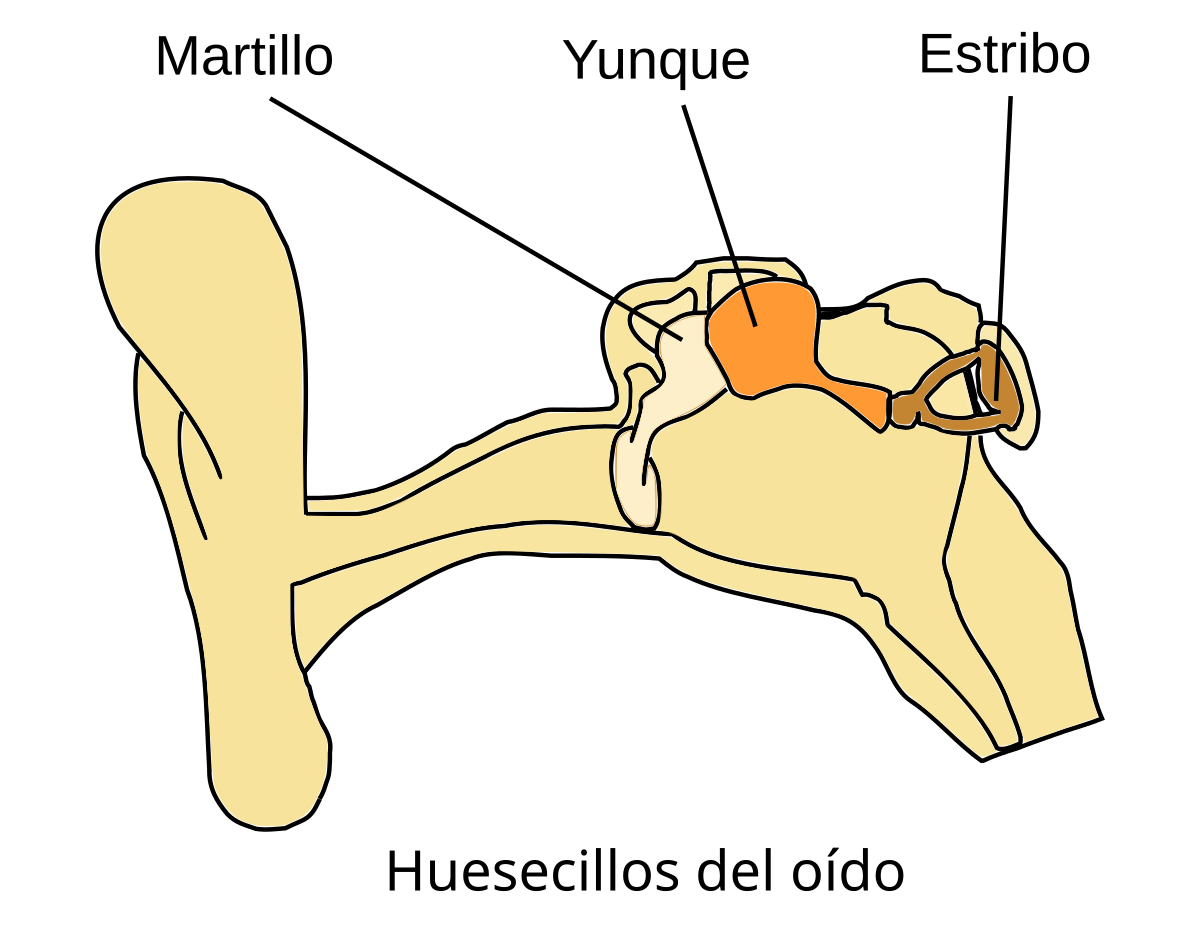
\includegraphics[width=0.6\textwidth]{figures/huesecillos.png}
    \caption{Diagrama de la cadena de huesecillos.}
    \label{huesecillos}
\end{figure}

\subsection{Tercera Ley (Acción y reacción)}
A toda acción le corresponde una reacción de igual magnitud pero con sentido opuesto. En una onda sonora, las moléculas de aire empujan a sus vecinas, que a su vez empujan de vuelta, transmitiendo el sonido en cadena.

\begin{quote}
    \textbf{Ejemplo clínico.} Cuando el estribo empuja la ventana oval en el oído interno, el líquido de la cóclea ejerce una fuerza opuesta. Esto transfiere la energía sonora al oído interno, donde se convierte en señales eléctricas.
\end{quote}

\subsection{Fricción y atenuación}
A medida que el sonido viaja, la fricción entre las moléculas de aire convierte parte de la energía en calor, reduciendo la intensidad del sonido. Este fenómeno, llamado \emph{atenuación}, es mayor en frecuencias altas (como los sonidos agudos de un silbido) y en ambientes húmedos.

\begin{quote}
    \textbf{Ejemplo práctico.} Los sonidos agudos de una voz se debilitan más rápido que los graves al viajar por el aire, lo que explica por qué escuchamos mejor los graves a la distancia.
\end{quote}

\begin{figure}[h]
    \centering
    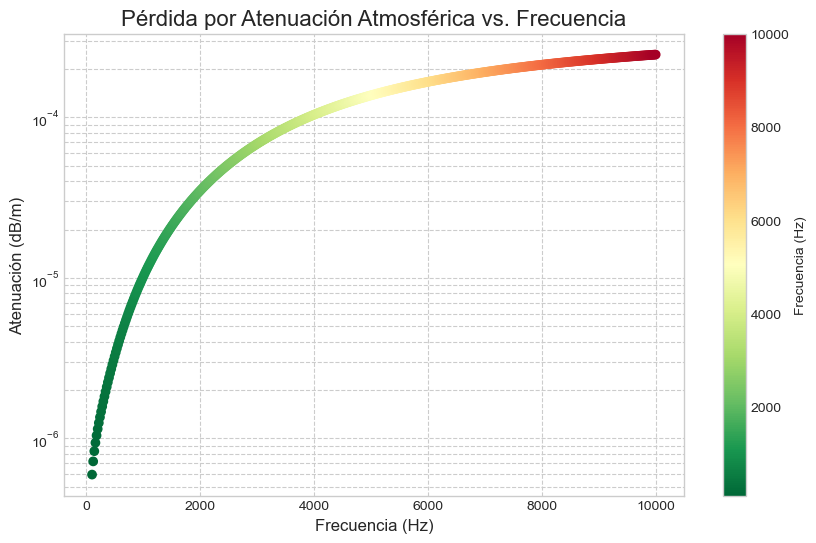
\includegraphics[width=0.8\textwidth]{figures/atenuacion_atmosferica.png}
    \caption{Fenómeno de atenuación atmosféroca.}
    \label{atenuacion_atmosferica}
\end{figure}


\section{Termodinámica del sonido}

La termodinámica estudia cómo la energía del sonido se transforma y se dispersa en el entorno. Esto es clave para entender cómo el sonido llega al oído y cómo se controla en entornos clínicos.

\subsection{Primera Ley: Conservación de la energía}
La energía no se crea ni se destruye, solo se transforma. En una onda sonora, la energía pasa de potencial (compresión del aire) a cinética (movimiento de partículas) y viceversa.

\begin{quote}
    \textbf{Ejemplo clínico.} En la cóclea, la energía mecánica del sonido (vibraciones del líquido) se transforma en energía eléctrica al activar las células ciliadas, que envían señales al cerebro.
\end{quote}

\subsection{Segunda Ley: Entropía y dispersión}
La entropía mide el desorden de un sistema. En acústica, la energía sonora tiende a dispersarse, lo que causa ecos y pérdida de claridad en espacios reverberantes. Por eso, las cabinas audiométricas están diseñadas para minimizar reflejos y mantener el sonido puro.

\begin{quote}
    \textbf{Ejemplo clínico.} En una cabina audiométrica, las paredes absorben el sonido para evitar ecos, asegurando que los tonos de la audiometría sean claros y precisos.
\end{quote}

\subsection{Temperatura y velocidad del sonido}
La velocidad del sonido depende de la temperatura del medio. En el aire, a 20°C, el sonido viaja a unos 343 m/s, pero aumenta aproximadamente 0.6 m/s por cada °C. En medios más densos, como el agua, la velocidad es mayor (1500 m/s).

\begin{table}[h]
    \centering
    \begin{tabular}{|l|c|l|}
        \hline
        \textbf{Condición} & $c$ (m/s) & \textbf{Observaciones} \\
        \hline
        $-10$~\textdegree C (aire seco) & 325 & Sonidos más apagados por alta atenuación \\
        0~\textdegree C & 331 & Referencia estándar \\
        20~\textdegree C, 50\%~RH & 343 & Condición típica en laboratorios \\
        35~\textdegree C, 90\%~RH & 352 & Mejora la inteligibilidad en exteriores \\
        \hline
    \end{tabular}
    \caption{Velocidad del sonido bajo distintas condiciones ambientales.}
\end{table}

\begin{quote}
    \textbf{Curiosidad.} Si inhalas helio, tu voz suena aguda porque el sonido viaja más rápido en helio (1000 m/s), cambiando las resonancias de tu garganta.
\end{quote}

\section{Ejemplos prácticos y autoevaluación}

\subsection{Problema resuelto: Reflejo estapedial}
El reflejo estapedial se activa a 85~dB~SPL, reduciendo el nivel a 79~dB~SPL. Calcula qué fracción de la energía acústica inicial se disipa o refleja.

\begin{quote}
    \textbf{Solución.} La diferencia es $\Delta L = 85 - 79 = 6$ dB. Esto significa que la intensidad se reduce a:
    \[
    \frac{I_2}{I_1} = 10^{-\Delta L/10} = 10^{-6/10} \approx 0.25.
    \]
    Se disipa o refleja el 75\% de la energía inicial, protegiendo el oído interno.
\end{quote}

\subsection{Ejemplo práctico: Vibración del tímpano}
El tímpano vibra con una fuerza de 0.001 N debido a un tono de 60 dB. Si su masa es aproximadamente 0.01 g (0.00001 kg), calcula la aceleración:
\[
a = \frac{F}{m} = \frac{0.001}{0.00001} = 100~\text{m/s}^2.
\]
Esto muestra cómo una pequeña fuerza produce un movimiento rápido en el tímpano.

\subsection{Ejercicios propuestos}
\begin{enumerate}
    \item \textbf{Gradiente térmico.} Dos impulsos sonoros se emiten a 500 m de distancia. En la mitad del trayecto, un frente cálido aumenta la temperatura de 20°C a 35°C. Calcula la diferencia en los tiempos de llegada. (\emph{Pista}: Usa $c = 343$ m/s a 20°C y $c = 352$ m/s a 35°C.)
    \item \textbf{Atenuación.} Un tono de 10 kHz pierde 0.2 dB por metro en aire húmedo. ¿Cuánto se atenúa tras viajar 10 m? (\emph{Solución}: 2 dB.)
    \item \textbf{Reflexión.} Explica cómo la tercera ley de Newton se aplica al movimiento de los huesecillos en el oído medio.
\end{enumerate}

\subsection{Preguntas de reflexión}
\begin{enumerate}
    \item ¿Por qué las frecuencias bajas (como un tambor) se escuchan a mayor distancia que las altas (como un silbido)?
    \item ¿Cómo ayuda una cabina audiométrica a reducir la entropía del sonido? Piensa en un consultorio con eco.
\end{enumerate}

\section{Glosario rápido}
\begin{description}
    \item[\textbf{Atenuación:}] Pérdida de intensidad del sonido debido a la fricción o dispersión en el medio.
    \item[\textbf{Entropía:}] Medida del desorden; en acústica, se relaciona con la dispersión de la energía sonora.
    \item[\textbf{Fuerza:}] Causa del movimiento, como la presión sonora que mueve el tímpano (medida en newtons, N).
    \item[\textbf{Inercia:}] Propiedad de un cuerpo para mantener su estado de reposo o movimiento.
\end{description}

\section{Resumen}
\begin{itemize}
    \item \textbf{Leyes de Newton:} Explican cómo las fuerzas del sonido mueven el tímpano y los huesecillos, esenciales para la audición.
    \item \textbf{Termodinámica:} La energía sonora se transforma (mecánica a eléctrica) y se dispersa (entropía), afectando la claridad del sonido.
    \item \textbf{Temperatura:} Afecta la velocidad del sonido (343 m/s a 20°C en aire), influyendo en la percepción y las pruebas audiométricas.
    \item \textbf{Atenuación:} Las frecuencias altas se debilitan más rápido, afectando la inteligibilidad a distancia.
\end{itemize}




\textbf{Recurso externo recomendado.} Video: \href{https://www.youtube.com/watch?v=3Br66N7QHpM&ab_channel=It%27sAumSumTime}{Why does sound travel faster in summer than in winter?.}

\bigskip
\noindent\emph{Conclusión.} Las leyes de Newton explican cómo el sonido mueve las estructuras del oído, desde el tímpano hasta la cóclea, mientras que la termodinámica nos ayuda a entender cómo la energía sonora se transforma y se pierde en el entorno. Estos principios son fundamentales para interpretar audiometrías, diseñar cabinas sonoamortiguadas y analizar cómo el ambiente afecta la voz y la audición. En la próxima unidad, exploraremos las ondas sonoras en detalle, conectándolas con la percepción auditiva.



%%%%%%%%%%%%%%%%%%%%%%%%%%%%%%%%%%%%%%%%%%%%%%%%%%%%%%%%%%%%%%%%%%%%%%%%%%%%%%%%%%%%%%%%%%%%%%%%%%
